%%%%%%%%%%%%%%%%%%%%%%%%%%%%%%%%%%%%%%%%%%%%%%%%%%%%%%%%%%%%%%%%%%%%%%%%%%%%%%%
%%%%%%%%%%%%%%%%%%%%%%%%%%%%%%%%%%%%%%%%%%%%%%%%%%%%%%%%%%%%%%%%%%%%%%%%%%%%%%%
%%%%%%%%%%%%%%%%%%%%%%%%%%%%%%%%%%%%%%%%%%%%%%%%%%%%%%%%%%%%%%%%%%%%%%%%%%%%%%%
%%%%%%%%%%%%%%%%%%%%%%%%%%%%%%%%%%%%%%%%%%%%%%%%%%%%%%%%%%%%%%%%%%%%%%%%%%%%%%%
\chapter{Introduction}
\label{ch:intro}
%%%%%%%%%%%%%%%%%%%%%%%%%%%%%%%%%%%%%%%%%%%%%%%%%%%%%%%%%%%%%%%%%%%%%%%%%%%%%%%
%%%%%%%%%%%%%%%%%%%%%%%%%%%%%%%%%%%%%%%%%%%%%%%%%%%%%%%%%%%%%%%%%%%%%%%%%%%%%%%
%%%%%%%%%%%%%%%%%%%%%%%%%%%%%%%%%%%%%%%%%%%%%%%%%%%%%%%%%%%%%%%%%%%%%%%%%%%%%%%
%%%%%%%%%%%%%%%%%%%%%%%%%%%%%%%%%%%%%%%%%%%%%%%%%%%%%%%%%%%%%%%%%%%%%%%%%%%%%%%

A social insect society is formed by thousands of individuals that continuously interact with each other inside a dark nest. 
Honey bees are organized in colonies, which are a complex and dynamic system.
Observing individual honey bees and their interactions with each other is vital for understanding collective behavior and the organization of tasks within the colony.

Within the BeesBook project of the Biorobotics Lab of Freie Universität Berlin, \textcite{wario2015automatic} developed technologies to automatically track all individuals of a honey bee (Apis mellifera) colony that are inside the honeycomb.
Shortly after hatching, each bee is marked with a circular 12-bit tag (Figure~\ref{fig:markers}) on their thorax and then added to the observation colony.
Several cameras observe the colony over a period of nine weeks. An image analysis pipeline evaluates each frame automatically. The resulting data set contains the exact position of each detected bee on the honeycomb and its age for each frame.

\begin{figure}[b]
	\centering
	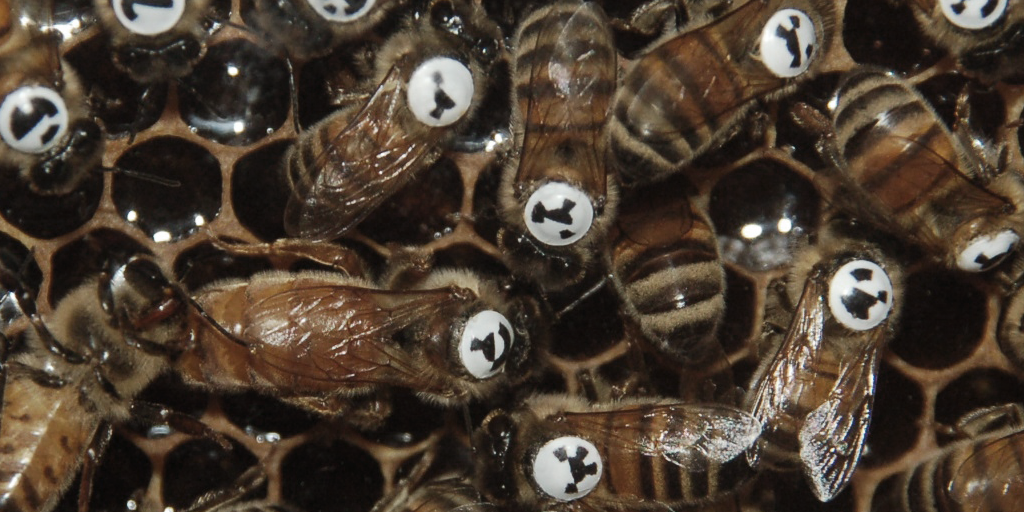
\includegraphics[width=1.0\textwidth]{Figures/markers}
	\caption{Tagged bees inside the observation hive.}
	\label{fig:markers}
\end{figure}

In this thesis, worker-worker interaction networks, based on spatial proximity, are derived from the described data set. Each node in the network is a bee and a link between two nodes results if two bees are located close to each other for a specified period.
The networks are time-aggregated, which means that one network represents the data of multiple frames.
After extracting the static networks, social network analysis methods are applied to determine the characteristics of the resulting networks and its social structure.

%%%%%%%%%%%%%%%%%%%%%%%%%%%%%%%%%%%%%%%%%%%%%%%%%%%%%%%%%%%%%%%%%%%%%%%%%%%%%%%
%%%%%%%%%%%%%%%%%%%%%%%%%%%%%%%%%%%%%%%%%%%%%%%%%%%%%%%%%%%%%%%%%%%%%%%%%%%%%%%
\section{Motivation}
\label{sec:intro:motivation}
%%%%%%%%%%%%%%%%%%%%%%%%%%%%%%%%%%%%%%%%%%%%%%%%%%%%%%%%%%%%%%%%%%%%%%%%%%%%%%%
%%%%%%%%%%%%%%%%%%%%%%%%%%%%%%%%%%%%%%%%%%%%%%%%%%%%%%%%%%%%%%%%%%%%%%%%%%%%%%%
Manual insect tagging and tracking is widely applied in the behavioral sciences.
Animals are marked using colored paint or numbered tags to distinguish individuals and then they are observed using a video recorder or by taking photos.
The interaction data is obtained by repeatedly watching the video files and manually extracting events.
Consequently, labeling only a subset of the colonies' individuals, short observation periods, a low sampling resolution, or limiting the observation to only a small area of the hive is very common.
Most insect related studies, in the field of animal social network analysis, analyze only a limited subset of the life of a colony.
Due to technical limitations, the majority of social insect interaction networks studies aggregate temporal tracking data into a single static network~\cite[Chapter~15]{krause2014animal}.

Recently, automated tracking of insects has become technically feasible~\cite{wario2015automatic, crall2015beetag, fiala2005comparing}.
Using automated high resolution tracking data, which includes all individuals of the complete hive over an extended period, allows for more advanced analysis focusing on temporal dynamics.
[TODO: some better motivation]


%%%%%%%%%%%%%%%%%%%%%%%%%%%%%%%%%%%%%%%%%%%%%%%%%%%%%%%%%%%%%%%%%%%%%%%%%%%%%%%
%%%%%%%%%%%%%%%%%%%%%%%%%%%%%%%%%%%%%%%%%%%%%%%%%%%%%%%%%%%%%%%%%%%%%%%%%%%%%%%
\section{Research Goal and Method}
\label{sec:intro:goals}
%%%%%%%%%%%%%%%%%%%%%%%%%%%%%%%%%%%%%%%%%%%%%%%%%%%%%%%%%%%%%%%%%%%%%%%%%%%%%%%
%%%%%%%%%%%%%%%%%%%%%%%%%%%%%%%%%%%%%%%%%%%%%%%%%%%%%%%%%%%%%%%%%%%%%%%%%%%%%%%
The aim of this thesis is to investigate whether the BeesBook data of tracked honey bees is useful for creating worker-worker interaction networks using spatial proximity as an indicator for interactions between bees.
Thus, I will implement a pipeline to extract networks out of the given data. Furthermore, I will investigate if the resulting networks are suitable for social network analysis.

I want to achieve my research goals by answering the following questions:

\begin{enumerate}
\item \emph{Is it possible to infer temporal networks with the provided honey bee tracking data?}\\
What challenges and limitations arise from using this data?
What pipeline parameters are necessary?
\item \emph{What kind of worker-worker interaction networks emerge and how are they structured?}\\
What is their topology?
What are the properties of the networks and how do they differ from randomly generated networks?
\item \emph{Does the network display a meaningful community structure?}\\
How are the identified communities characterized?
Do they reflect already known colony behavior concerning age and spatial distribution?
\item \emph{How do these communities develop over time?}\\
Do the communities have stable properties?
How do members move between communities?
\end{enumerate}


This work is meant to establish the foundation for future research using a network science approach to study the complex system of honey bee colonies and their collective behavior.

The methodology of this work consists of two parts, described in detail in Chapter~\ref{ch:approach}.
The first part details the approach to infer and define spatial proximity networks using the honey bees tracking data.
The second part analyzes properties, communities, and the development of the identified networks.  

\section{Outline}
This thesis is organized as follows.
Chapter~\ref{ch:foundation} is a short introduction into social network analysis (SNA). I define network measures, terms, and algorithms used throughout this work and provide a brief summary of the current state of research concerning social insect networks, temporal networks and community detection in animal social networks.
In Chapter~\ref{ch:approach} I describe my research approach in general and how the pipeline infers networks out of the given dataset, what steps are needed and what parameters it uses.
Also, I explain and justify what decisions I took during the network analyses and community detection process.
In Chapter~\ref{ch:results}, I report the results of the network analysis and the characteristics of the extracted communities.
Finally, in chapter~\ref{ch:conclusion}, I summarize the results, discuss limitations and conclude with directions for future work.